\PassOptionsToPackage{french,dutch,english}{babel}
\documentclass[twoside]{extreport}

\usepackage{flanders_report}
\codesize{\footnotesize}




\title{Ondersteuningsproject bij de uitvoering van de reemonitoring in het
Zonienwoud}
\subtitle{Jaarlijks rapport - referentieperiode: 2008-2019}
\author{Niko Boone, Jim Casaer, Jan Vercammen, Céline Malengreaux, Alain Licoppe}

\reportnumber{doi.org/10.21436/inbor.17589206}




% Alter some LaTeX defaults for better treatment of figures:
% See p.105 of "TeX Unbound" for suggested values.
% See pp. 199-200 of Lamport's "LaTeX" book for details.
%   General parameters, for ALL pages:
\renewcommand{\topfraction}{0.9}	% max fraction of floats at top
\renewcommand{\bottomfraction}{0.8}	% max fraction of floats at bottom
%   Parameters for TEXT pages (not float pages):
\setcounter{topnumber}{2}
\setcounter{bottomnumber}{2}
\setcounter{totalnumber}{4}     % 2 may work better
\setcounter{dbltopnumber}{2}    % for 2-column pages
\renewcommand{\dbltopfraction}{0.9}	% fit big float above 2-col. text
\renewcommand{\textfraction}{0.07}	% allow minimal text w. figs
%   Parameters for FLOAT pages (not text pages):
\renewcommand{\floatpagefraction}{0.7}	% require fuller float pages
% N.B.: floatpagefraction MUST be less than topfraction !!
\renewcommand{\dblfloatpagefraction}{0.7}	% require fuller float pages

\begin{document}
\maketitle
\pagenumbering{arabic}



\chapter*{}\label{section}
\addcontentsline{toc}{chapter}{}

\chapter*{Dankwoord}\label{dankwoord}
\addcontentsline{toc}{chapter}{Dankwoord}

Het uitvoeren van de tellingen waarover gerapporteerd wordt in dit
rapport, was niet mogelijk zonder de inzet van talloze vrijwilligers
afkomstig uit allerlei organisaties en verenigingen. We willen dan ook
iedereen bedanken voor de medewerking.

Voor de hulp bij de praktische organisatie bedanken we graag iedereen
die hieraan meewerkte bij het Agentschap voor Natuur- en Bos (ANB),
Leefmilieu Brussel (BIM), de Service Public de Wallonie (SPW) en het
Instituut voor Natuur- en Bosonderzoek (INBO).


\clearpage

\phantomsection
\setcounter{tocdepth}{4}
\tableofcontents
\addcontentsline{toc}{chapter}{\contentsname}

  


\clearpage


\chapter{Inleiding}\label{inleiding}

Het ree ( \emph{Capreolus capreolus} ) is een van de grootste zoogdieren
in het Zonienwoud. De soort is in elk deel van het woud aanwezig, maar
met wisselende dichtheden.

Om een zicht te krijgen op de evolutie van de reepopulatie in het
volledige Zonienwoud, dus over de drie gewesten heen, voeren het
Agentschap voor Natuur- en Bos (ANB), Leefmilieu Brussel (BIM), de
Service Public de Wallonie (SPW) en het INBO sinds 2008 jaarlijks
systematische tellingen uit in het Zoni?nmassief. De vzw Wildlife \& Man
stond in voor de voorbereidende studies en blijft betrokken bij de
jaarlijkse terugkoppelingsmomenten.

Het is al lang gekend dat het tellen van alle reeen in een gebied niet
mogelijk of moeilijk haalbaar is. Veranderingen of trends binnen een
reepopulatie zijn daarentegen wel goed meet- en opvolgbaar.
Wetenschappelijk onderzoek uit Frankrijk toonde aan dat de
kilometerindex methode (KI) toelaat om met zekerheid te bepalen of een
reepopulatie in een gegeven bosgebied toeneemt, afneemt of stabiel
blijft. Deze methode werd in het Zoni?nwoud in 2008 opgestart
\citep{Vercammen2011}.

Dit rapport omvat een korte beschrijving van de KI-methodologie en geeft
de resultaten weer voor de periode 2008-2019. Het rapport is een vervolg
op gelijkaardige rapporten uit voorgaande jaren.

\chapter{De kilometerindex (KI) in het
Zonienwoud}\label{de-kilometerindex-ki-in-het-zonienwoud}

\section{Methodologie}\label{methodologie}

Het principe van de kilometerindex bestaat erin jaarlijks een aantal
vaste parcours \ref{fig:telparcours} af te stappen en het aantal
waargenomen reeen langs het parcours te tellen. Door vervolgens het
aantal reeen te delen door de afgelegde afstand, bekom je een relatieve
kilometerindex (het aantal geobserveerde reeen per kilometer). Om uit de
index op een statistisch verantwoorde manier conclusies te trekken, zijn
jaarlijks minstens 3 a 4 telsessies noodzakelijk. Die worden liefst
binnen een zo kort mogelijke periode uitgevoerd. Per telsessie worden
alle parcours afgestapt. Dat gebeurt bij voorkeur simultaan op dezelfde
ochtenden of avonden. Na elke telsessie wordt eerst de kilometerindex
per parcours berekend, vervolgens de gemiddelde kilometerindex over alle
parcours. Door deze procedure een aantal keer per jaar te herhalen,
wordt een jaarlijks gemiddelde bekomen. Op dit gemiddelde kan een
betrouwbaarheidsinterval worden berekend. Deze manier van werken laat
toe om op een statistisch verantwoorde manier de gemiddelden over een
tijdsperiode te vergelijken. Voor meer informatie over deze methode
verwijzen we naar \citet{Malengreaux2008}. De eerste resultaten zijn
terug te vinden in het rapport `Reewildtellingen' \citep{Vercammen2011},
de daaropvolgende verslagen op de website van het INBO
(\url{http://www.inbo.be}) en onder de hoofding ``Documenten'' op de
website \url{http://www.wildlifeandman.be}.

\begin{figure}

{\centering 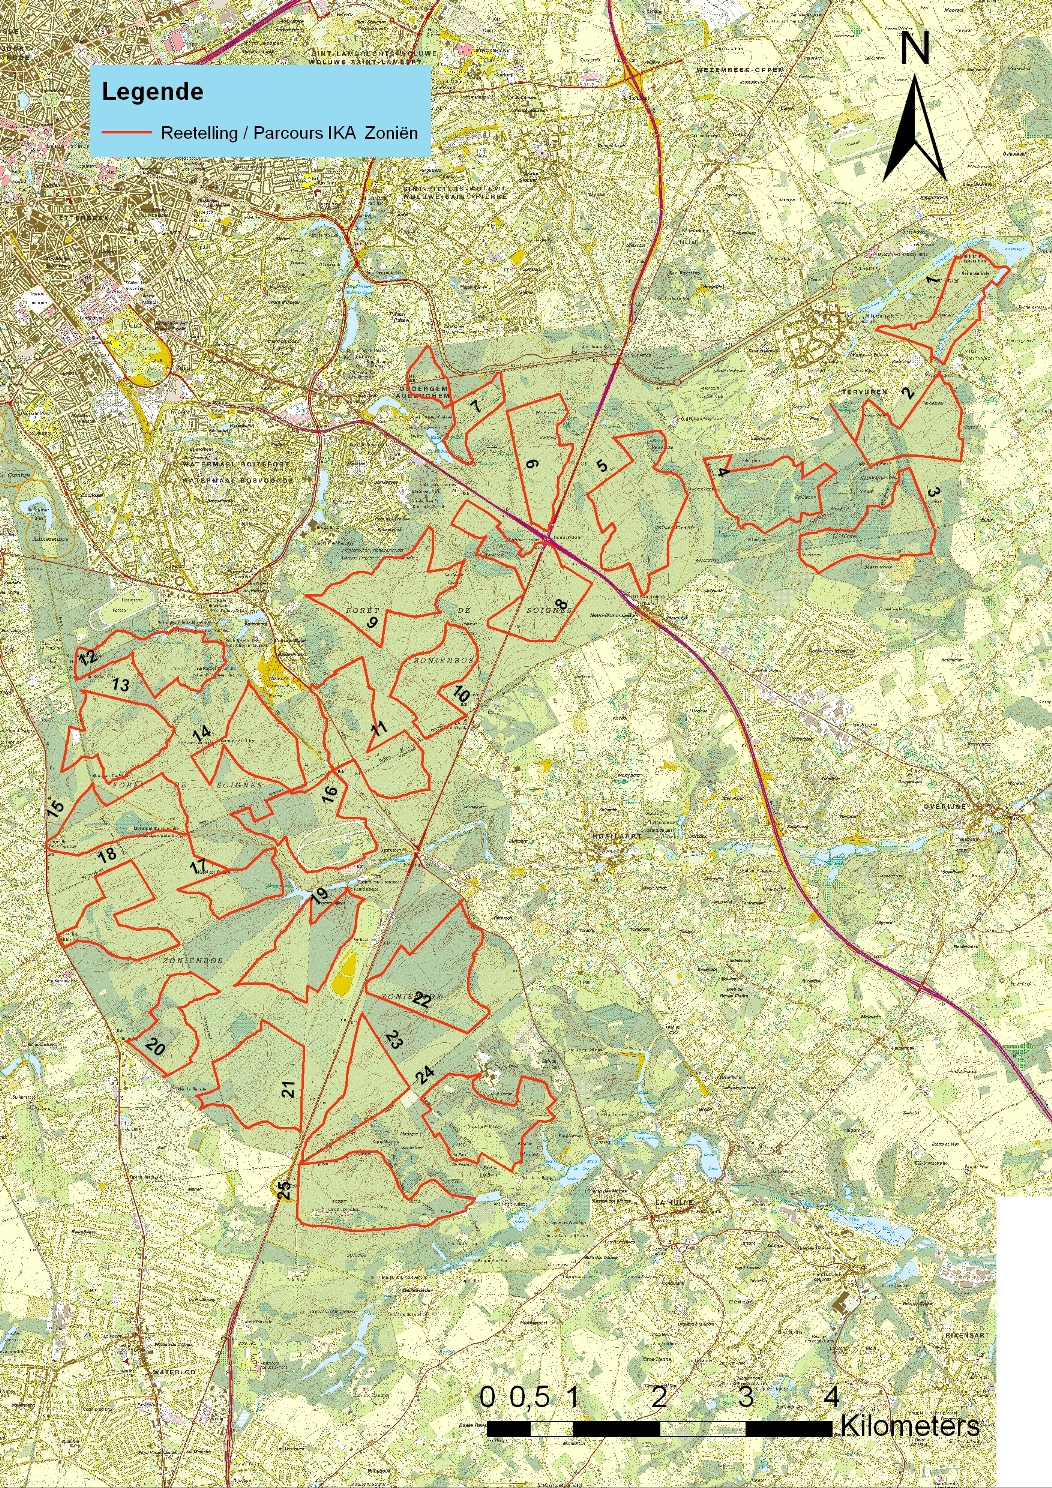
\includegraphics[width=2.05in]{afbeeldingen/telparcours} 

}

\caption{Overzicht van de verschillende telparcours in het Zonienwoud. Parcours nummer 1 werd enkel in 2008 geteld.}\label{fig:telparcours}
\end{figure}

\chapter{Resultaten}\label{resultaten}

\section{Aantal kilometer parcours
afgelegd}\label{aantal-kilometer-parcours-afgelegd}

In het verkennend aanvangsjaar 2008 werden er vier ochtend- en vier
avondtellingen uitgevoerd. Sinds 2009 vinden de tellingen enkel 's
ochtends plaats. Er wordt een keer per week geteld gedurende vier
opeenvolgende weken. De 24 telparcours zijn samen 118,5 km lang. In
principe wordt dus jaarlijks 473 km afgelegd. In 2016, 2017 en 2019
werden enkele trajecten een of meerdere keren niet geteld omdat er
onvoldoende tellers aanwezig waren. In totaal gaat het om acht parcours.
Sinds de start van het project werd in het kader van deze
populatie-opvolging al 6142 km gewandeld.

\section{Maximaal en minimaal aantal waargenomen reeen per
jaar}\label{maximaal-en-minimaal-aantal-waargenomen-reeen-per-jaar}

Tabel 1 geeft per jaar de telsessie aan met het hoogste en deze met het
laagste aantal waargenomen reeen. De lage aantallen in 2014/2015 en
2016/2017 waren mogelijk het gevolg van respectievelijk mist en zware
buien tijdens de betreffende telling. In 2019 zijn tijdens de telsessie
met het laagste aantal waargenomen ree?n, twee trajecten niet geteld.
Tijdens de telsessie met het hoogste aantal waargenomen reeen is een
traject niet geteld.

\section{Evolutie van de kilometerindex van 2008 tot
2019}\label{evolutie-van-de-kilometerindex-van-2008-tot-2019}

De telresultaten van 2019 bevestigen de tendens van de laatste jaren. Na
het opstartjaar 2008 kunnen we duidelijk twee verschillende perioden
onderscheiden. Een eerste periode, van 2009 tot en met 2013, vertoont
een relatief stabiel beeld met een gemiddeld aantal van meer dan 0,9
waargenomen ree?n per gewandelde kilometer. In de tweede periode, van
2014 tot en met 2019, ligt het jaarlijks gemiddelde onder de 0,9
waargenomen reeen per kilometer en lijkt het erop dat er na een periode
van afnemende aantallen nu een nieuwe stabiele toestand is (geen dalende
trend meer), zij het wel op een duidelijk lager niveau dan in de periode
tot 2013.

\section{Evolutie van de kilometerindex per parcours in
2019}\label{evolutie-van-de-kilometerindex-per-parcours-in-2019}

Wanneer we per parcours de tellingen van dit jaar vergelijken met de
mediaan van de voorbije jaren (2008 - 2018), dan zien we drie fenomenen:
1. bij negen trajecten is de KI bij alle tellingen van dit jaar lager
dan de mediaan van de vorige jaren (parcours 3, 5, 6 7, 14, 18, 21, 23
en 24); 2. bij 18 parcours zijn op een of meer teldagen geen reeen
waargenomen; 3. bij 15 trajecten waren er dagen waarop het aantal
waargenomen reeen boven de mediaan van de vorige jaren lag. (figuur 4).

Wanneer we per parcours de gemiddelde KI voor 2019 vergelijken met de
mediaan uit de periode van 2008 tot en met 2013, dus voor de
opmerkelijke terugval, dan zien we dat de daling van de KI zich in bijna
alle trajecten heeft voorgedaan (figuur 5). Enkel in zeven van de 24
trajecten oversteeg het gemiddelde in 2019 de mediaan voor de periode
2008-2013. Bij 9 trajecten ligt het volledige betrouwbaarheidsinterval
van de KI van 2019 onder de mediaan voor de periode 2008-2013. Dat wijst
voor deze trajecten op een significante daling sinds 2013.

\section{Duur van de tellingen}\label{duur-van-de-tellingen}

De ideale duur voor het uitvoeren van een telling is 1.30 uur tot 1.45
uur. Met uitzondering van 2011 voldeed de gemiddelde duur hier aan.
(tabel 2). Hoewel de gemiddelde duur van een telling de laatste jaren
licht stijgt, blijven er tellingen waarbij de teller maar een uur
onderweg was. Snel wandelen kan de waarnemingskans van reeen sterk laten
dalen. Het voldoende tijd nemen voor een telling blijft een
aandachtspunt.

\section{Oorzaken van de veranderingen in het aantal waargenomen
ree?n}\label{oorzaken-van-de-veranderingen-in-het-aantal-waargenomen-reen}

De lagere aantallen waargenomen ree?n kunnen zowel het gevolg zijn van
i) een effectief lager aantal reeen als ii) van een verminderde
waarnemingskans. Onder waarnemingskans verstaan we de waarschijnlijkheid
dat een aanwezige ree ook effectief waargenomen wordt. Een verminderde
waarnemingskans kan zowel aan een verandering in het gedrag van de reeen
te wijten zijn, als aan een verminderde zichtbaarheid door de
aanwezigheid van meer dekking (struiken en jonge bomen).

\subsection{Lager aantal ree?n}\label{lager-aantal-reen}

Bij een ongewijzigde waarnemingskans betekent het lager aantal
waargenomen ree?n per kilometer dat het aantal ree?n in het Zonienwoud
daalt. Mogelijke oorzaken daarvan zijn lagere voortplanting, hogere
sterfte en/of emigratie. Omdat in het Zonienwoud geen jacht plaatsvindt,
zou een hogere mortaliteit veroorzaakt kunnen worden door een toename
van ziektes, predatie, verkeersslachtoffers of loslopende honden. We
beschikken echter niet over gegevens over de dood gevonden dieren of
over de populatiegegevens van mogelijke predatoren in en rond het
Zonienwoud. Er wordt ook niet systematisch onderzoek naar gedaan. We
beschikken ook niet over de nodige gegevens om de hypotheses van lagere
geboortecijfers (aantal embryo's per drachtige geit en het aandeel
drachtige geiten) of plotse sterke emigratie te kunnen onderzoeken. Ook
de vraag of een mogelijke wijziging in recreatiedruk een effect heeft,
blijft momenteel onbeantwoord. Een verhoogde recreatiedruk kan
resulteren in een emigratie naar rustigere stukken in of buiten het bos,
of in een verandering in het gedrag van de reeen. Een eerste stap om dit
te onderzoeken is de evolutie nagaan van het aantal recreanten dat
jaarlijks het Zonienwoud bezoekt en/of van de dichtheid van het netwerk
aan paden in het boscomplex. Binnen het kader van dit project is deze
opvolging echter niet voorzien.

\subsection{Verandering van de zichtbaarheid op de
trajecten}\label{verandering-van-de-zichtbaarheid-op-de-trajecten}

Bij een bos dat niet onderhevig is aan sterke veranderingen in beheer of
door andere externe factoren, wordt de vermindering in zichtbaarheid op
sommige trajecten in theorie gecompenseerd door een toename op andere
trajecten. Dit is zeker het geval in een groot gebied zoals het
Zoni?nwoud waar de parcours homogeen over het volledige gebied verdeeld
zijn. Omdat er in de telperiode 2008-2015 geen metingen uitgevoerd zijn
om eventuele veranderingen in de zichtbaarheid aan te tonen, is het niet
mogelijk het potenti?le effect ervan in te schatten. Om toch te proberen
hier een idee over te krijgen, voerden we in 2015 een bevraging uit bij
alle tellers. Het resultaat daarvan is besproken in het
opvolgingsrapport 2015 (Huysentruyt et al., 2015). Om het effect van
veranderingen in zichtbaarheid te kunnen modelleren en op te volgen naar
de toekomst toe, werd besloten de zichtbaarheid op de verschillende
trajecten effectief te meten zie 3.6.3.

\subsection{Meten van de
waarnemingskans}\label{meten-van-de-waarnemingskans}

Om na te gaan in welke mate de vegetatie de zichtbaarheid van reeen
beinvloedt, voerden we in februari 2018 een zichtbaarheidsmeting uit
langs alle telparcours. Dit was een herhaling van de meting van november
2015. De zichtbaarheidsmeting gebeurt op volgende manier: Op elk van de
24 telparcours wordt om de 500 m, afwisselend links en rechts van de
weg, de zichtbaarheid geschat op 12,5 m, 25 m en 50 m. Dit gebeurt met
behulp van een 1,70 m lange meetlat, onderverdeeld in vakken van 10 cm
die alternerend geel en oranje van kleur zijn (figuur 6). Op de drie
afstanden wordt gekeken in welke mate de vegetatie deze vakken bedekt.
Elk van de 17 vakken krijgt een waarde 1 (volledig zichtbaar), 0,5
(deels zichtbaar) of 0 (niet zichtbaar). In totaal werden 221 locaties
gemeten. De meetlocaties van 2018 zijn dezelfde als deze uit 2016. Dit
is mogelijk omdat de co?rdinaten van de punten gekend zijn (zie
Huysentruyt et al., 2017).

Vervolgens wordt de score voor elk hoogte-interval gewogen met een
factor die het percentage weergeeft van een staand of liggend ree dat in
dit hoogte-interval in theorie zichtbaar is (voor een volledige
bespreking en de gebruikte correcties zie Casaer (2003)) (figuur 7).
Door de meting te herhalen kunnen we kijken of de waarnemingskans van
ree?n wijzigde in de tijd. Hoe denser de ondergroei, hoe moeilijker de
reeen waarneembaar zijn.

Wanneer we voor elk van de telparcours de situatie in 2015 vergelijken
met die van 2018 (figuur 8), zien we een relatieve verhoging van de
waarnemingskans op parcours 3 en een daling voor parcours 24. Op alle
andere parcours lijken er zich geen belangrijke wijzigingen te hebben
voorgedaan.

Deze meting, uitgevoerd door Quentin Jocque (Quentin, 2018) in het kader
van zijn masterthesis, laat toe te besluiten dat de waarnemingskans over
het algemeen niet gewijzigd is in 2,5 jaar. De gemiddelde
zichtbaarheidsscore voor heel het Zonienwoud is op de drie afstanden
vergelijkbaar tussen beide jaren (figuur 9). Dit was ook te verwachten
gezien de korte periode tussen beide metingen en het uitblijven van
gebeurtenissen die de zichtbaarheid plots kunnen wijzigen (bv.
stormschade, natuurbrand of grootschalige kappingen). Voor wat betreft
de waarnemingskans gelinkt aan de ondergroei in het bos, zijn de
reetellingen uit de periode 2016-2018 dus goed vergelijkbaar.

\chapter{\texorpdfstring{Schatting van de reepopulatie met behulp van
\emph{distance
sampling}}{Schatting van de reepopulatie met behulp van distance sampling}}\label{schatting-van-de-reepopulatie-met-behulp-van-distance-sampling}

Het uitgangspunt bij distance sampling is dat de waarschijnlijkheid om
een dier waar te nemen daalt in functie van de afstand tussen de
waarnemer en het dier (Buckland et al., 2001). De methode bestaat erin
de loodrechte afstand te bereken tussen het waargenomen dier en het
telparcours. Dit wordt gedaan door de afstand tussen de waarnemer en
dier te meten (met een afstandsmeter) zowel als de hoek van deze lijn
t.o.v. het telparcours (zie Casaer \& Malengreaux, 2008). Op basis van
deze gegevens kan de waarnemingskans in functie van de afstand
gemodelleerd worden; een functie die eigen is aan de diersoort en een
bepaald gebied/vegetatie (figuur 10). Deze functie kan op zijn beurt
gehanteerd worden om voor een bepaald gebied de densiteit van dieren te
berekenen.

\section{Methode}\label{methode}

In maart 2018 kreeg een deel van de tellers een afstandsmeter ter
beschikking. We beschikten echter over onvoldoende toestellen voor alle
24 tellers. Het gebruik van een betrouwbare afstandsmeter is een
voorwaarde om distance sampling toe te passen. In tegenstelling tot de
normale aanpak werd er gewerkt met de directe afstand tussen de
waarnemer en het geobserveerde dier en niet met de loodrechte afstand.

\section{Resultaten}\label{resultaten-1}

Met uitzondering van enkele waarnemingen op uitzonderlijk grote
afstanden, bedroeg de gemiddelde afstand tussen de waarnemer en een
ree/groep reeen over alle parcours heen 67 m. Figuur 11 toont de
gemiddelde waarnemingsafstand per telparcours.

\subsection{Problmen/knelpunten tijdens het
onderzoek}\label{problmenknelpunten-tijdens-het-onderzoek}

We beschikten over onvoldoende afstandsmeters om op alle telparcours
tegelijk metingen uit te voeren. De metingen gebeurden dus slechts in
een deel van het Zonienwoud. Bovendien volstond het aantal
waarnemingen/waargenomen reeen niet om een betrouwbare detectiefunctie
te berekenen. De gemeten afstanden zijn de directe afstanden tussen de
waarnemer/teller en de ree. Distance sampling vereist echter het gebruik
van de loodrechte afstand tussen het telparcours en het dier. Er moet
onderzocht worden of en hoe het gebruik van de directe afstand in plaats
van de loodrechte afstand de densiteitsschatting be?nvloedt.

Figuur 12 toont dat de meeste waarnemingen plaatsvonden op een afstand
tussen 40 en 80 m. Op basis van het theoretische model zou je echter
verwachten dat het maximum aantal waarnemingen vlak bij of op het
teltraject gebeuren. De verstoring door de waarnemer of de reactietijd
van de waarnemer tussen het ogenblik dat de ree beweegt en het moment
dat deze de ree ziet, kunnen verklaren dat er meer reeen gezien werden
op grotere afstand dan verwacht. Het softwarepakket Distance corrigeert
hiervoor bij de eerste afstandsintervallen wanneer het de
detectiefunctie inschat (zie figuur 13).

Door de vele methodologische vragen en problemen werd beslist de
berekeningen van de reedensiteit op basis van de gegevens van dit
pilootproject, niet op te nemen in dit rapport.

\chapter{Conclusies}\label{conclusies}

Na de daling van de gemiddelde kilometerindex die we in 2014, 2015 en
2016 vaststelden, lijkt de populatie zich nu te stabiliseren op een
lager niveau. Terwijl de gemiddelde KI in de periode 2008-2013 rond 1
ree/km schommelde, oversteeg de index sinds 2014 nooit 0,75. Sinds 2017
zakte de KI tot onder 0,6.

In 2016 haalden we al aan dat deze situatie zou kunnen wijzen op een
achteruitgang van de reepopulatie in het Zonienwoud. Om hier uitsluitsel
over te kunnen geven, is het nodig om de mogelijke oorzaken van de
achteruitgang te identificeren en om de nodige gegevens te verzamelen om
die hypotheses te kunnen onderzoeken. Voorbeelden van dergelijke
gegevens zijn: aantal aanrijdingen met ree?n, informatie over stroperij,
impact van loslopende honden, bio-indicatoren van de reepopulatie (bv.
aantal embryo's per drachtige geit, het aandeel drachtige geiten),
metingen van de recreatiedruk en gegevens over de aanwezigheid van
andere wilde hoefdieren. Binnen het kader van de huidige monitoring is
het in kaart brengen en opvolgen van deze mogelijke factoren echter niet
voorzien.

Om na te gaan of de waargenomen tendens een gevolg kan zijn van een
verminderde waarnemingskans, voerden we in 2015 een bevraging uit bij de
tellers. Bij hen bestond de perceptie dat de zichtbaarheid in het
algemeen verminderd is, wat geheel of gedeeltelijk de daling van de KI
zou kunnen verklaren. Een vergelijking van de zichtbaarheidsmetingen uit
2015 en 2018 toont weinig verschillen. De zichtbaarheid is gelijkaardig
in beide jaren. Dit was ook te verwachten gezien de korte periode tussen
beide metingen en het uitblijven van gebeurtenissen die de zichtbaarheid
plots kunnen wijzigen (bv. stormschade, natuurbrand of grootschalige
kappingen). Veranderingen in zichtbaarheid in het bos door veranderingen
in de vegetatie doen zich, zolang er geen calamiteiten optreden, normaal
gezien slechts op langere termijn voor.

%startbib
\cleardoublepage
\bibliographystyle{inbo}
\bibliography{literatuurlijst.bib}
\addcontentsline{toc}{chapter}{\bibname}
%endbib

\end{document}
